\documentclass[10pt]{article}
\usepackage[margin=0.8in]{geometry}
\usepackage{graphicx}
\usepackage{amsmath}
\usepackage[numbers]{natbib}

\graphicspath{{project5_symmetry/Report/images/}}
\linespread{1.0}
\setlength{\abovedisplayskip}{2pt}
\setlength{\belowdisplayskip}{2pt}
\setlength{\textfloatsep}{4pt plus 1pt minus 2pt}
\setlength{\floatsep}{4pt plus 1pt minus 2pt}
\setlength{\intextsep}{4pt plus 1pt minus 2pt}
\setlength{\parskip}{0pt}

\title{Landmark Symmetry and Cognitive Map Formation in Predictive Recurrent Neural Networks}
\author{Author Name\\Department or Program Affiliation}
\date{}

\begin{document}

\maketitle
\vspace{-1.2em}

\begin{abstract}
Representational similarity analysis (sRSA) is invariant to global map rotation -- permuting the rows of the hidden state matrix preserves all pairwise distances -- making it unable to detect orientational degeneracy across training seeds. To separate global from local failure modes, we developed three purpose-built metrics: Rotational Autocorrelation (RA) for unit-level aliasing, Permutation-Aware Alignment (PAA) for cross-seed orientational divergence, and C2 Contrast for group-theoretic structure in the population code. Applied to a NormReLU pRNN trained in C4-symmetric, C2-symmetric, and asymmetric arenas with matched observational discriminability (ODI = 0.336), we find: global orientational degeneracy did not occur (PAA gain < 0.01 in all conditions); local aliasing increased 2.7-fold in S4 relative to S1 (RA = 0.187 vs 0.069); and C2 symmetry group structure was encoded in the population code (C2 Contrast = +0.045). Landmark symmetry folds the representation and degrades metric geometry without destroying global map orientation, because head-direction input anchors oriented transition statistics even when visual observations are rotationally degenerate.
\end{abstract}

\section{Introduction}

Predictive learning explains hippocampal map formation as a state-estimation problem. A recurrent network trained to forecast future observations must retain latent variables that support path integration, and spatial structure can emerge without coordinate supervision \cite{levenstein2024}. Symmetric landmarks create an identification problem for this objective. If four arena quadrants generate identical landmark sequences up to rotation, then the prediction loss fails to distinguish globally rotated maps or merges rotationally equivalent locations into one representational class.

These outcomes have different computational costs. A globally degenerate map makes orientation arbitrary across training runs. A folded but globally stable map preserves a common frame while confusing positions that share the same landmark history. For navigation, the second failure mode predicts errors at symmetric goal locations rather than complete loss of map structure. The experiment therefore asks whether landmark diversity prevents map collapse or instead improves the precision of a map that predictive learning already stabilizes.

We test three conditions that differ only in landmark symmetry: S4 is C4-symmetric, S2 is C2-symmetric, and S1 is asymmetric. ODI is held fixed at 0.336, so all conditions contain the same total positional information. The analysis separates four questions that sRSA alone conflates: whether position is linearly decodable, whether neural distance follows Euclidean or city-block geometry, whether independent seeds choose incompatible global orientations, and whether the population code reflects the C2 symmetry relation. The central result is that symmetry degrades precision and geometry, but not global orientation.

A single map-quality score cannot separate these failure modes because sRSA is formally blind to global map rotation. The metric computes rank correlation over all pairwise neural distances; permuting the rows of H -- which corresponds to relabeling the global orientation of the learned map -- leaves every pairwise distance invariant. sRSA therefore returns identical values whether independent seeds learn a consistent global frame or arbitrary rotations of one another. Three purpose-built metrics address this gap. PAA (Permutation-Aware Alignment) tests whether a rotated alignment between seeds improves over the identity alignment, detecting global orientational divergence directly. RA (Rotational Autocorrelation) measures whether individual units respond at multiple rotationally equivalent positions, detecting local aliasing at the unit level. C2 Contrast compares neural similarity between 180-degree-related and 90-degree-related quadrant pairs, detecting whether the population code encodes the symmetry group of the observation function. This decomposition allows us to separate global orientational stability from local representational precision, which a single map quality score cannot do.

\section{Methods}

\subsection{Environment and Model}

The arena was an $18\times18$ grid with approximately 324 positions. This size gives enough samples for stable pairwise distance matrices while still allowing broad coverage in trajectories of length $T=200$. The visual field was $F=7$, large enough to capture local landmark geometry but too local to expose the full arena. The three landmark layouts were matched for observational discriminability,
\[
\mathrm{ODI}=1-\frac{H(X\mid O)}{H(X)}=0.336,
\]
where $X$ is position and $O$ is the egocentric observation. Holding this value fixed makes symmetry group $G$ the experimental variable: S4 has C4-equivalent observations, S2 has C2-equivalent observations, and S1 has no designed quadrant equivalence.

The model was a NormReLU pRNN with hidden dimension $N=128$. At time $t$ the recurrent state depended on egocentric observation $o_t$, action $a_t$, 12-bin head direction $d_t$, and previous state $h_{t-1}$:
\[
h_t=\mathrm{NormReLU}(W_h h_{t-1}+W_o o_t+W_a a_t+W_d d_t).
\]
Training minimized multi-step observation prediction over horizon $k=5$,
\[
\mathcal{L}=\sum_{j=1}^{k}\|\hat{o}_{t+j}-o_{t+j}\|_2^2,
\]
for 80,000 optimization steps. No coordinate labels entered the loss. Hidden states were analyzed after training as population codes $h(x)$ over arena positions. The head-direction input gives the transition model an oriented path-integration signal, so visual C4 symmetry does not imply rotational equivalence of the full input sequence (12-bin one-hot head-direction, Levenstein et al. Figure 4 [1]).

\subsection{Evaluation Protocol}

After training, hidden states were collected by evaluating the pRNN across arena positions and seeds. The analysis compared conditions at three levels: whether position could be read out from the population state, whether the population geometry matched Euclidean or city-block distance, and whether symmetry appeared as global map rotation or local folding. This organization matters because a single map-quality score cannot separate these failure modes. sRSA can show that hidden-state geometry is spatial, but decoding, cross-seed alignment, unit-level rotational aliasing, and dimensionality are needed to decide what kind of spatial representation was learned.

\section{Results}

\subsection{Summary Across Metrics}

Symmetry systematically degrades spatial precision and metric geometry without producing global orientational degeneracy: sRSA falls from 0.745 in S1 to 0.647 in S4, decoding error rises from 0.365 to 0.524, and DTG grows more negative (−0.020 to −0.052), while cross-seed alignment remains above 0.97 in all conditions (Figure 1). The summary table in Figure~\ref{fig:summarytable} gives the corresponding values: sRSA Euclid is 0.647 in S4, 0.657 in S2, and 0.745 in S1; decoding error is 0.524, 0.475, and 0.365. Matched ODI therefore does not imply matched representation. The same amount of sensory information produces different population codes when the equivalence structure of the observations changes.

\begin{center}
\centering
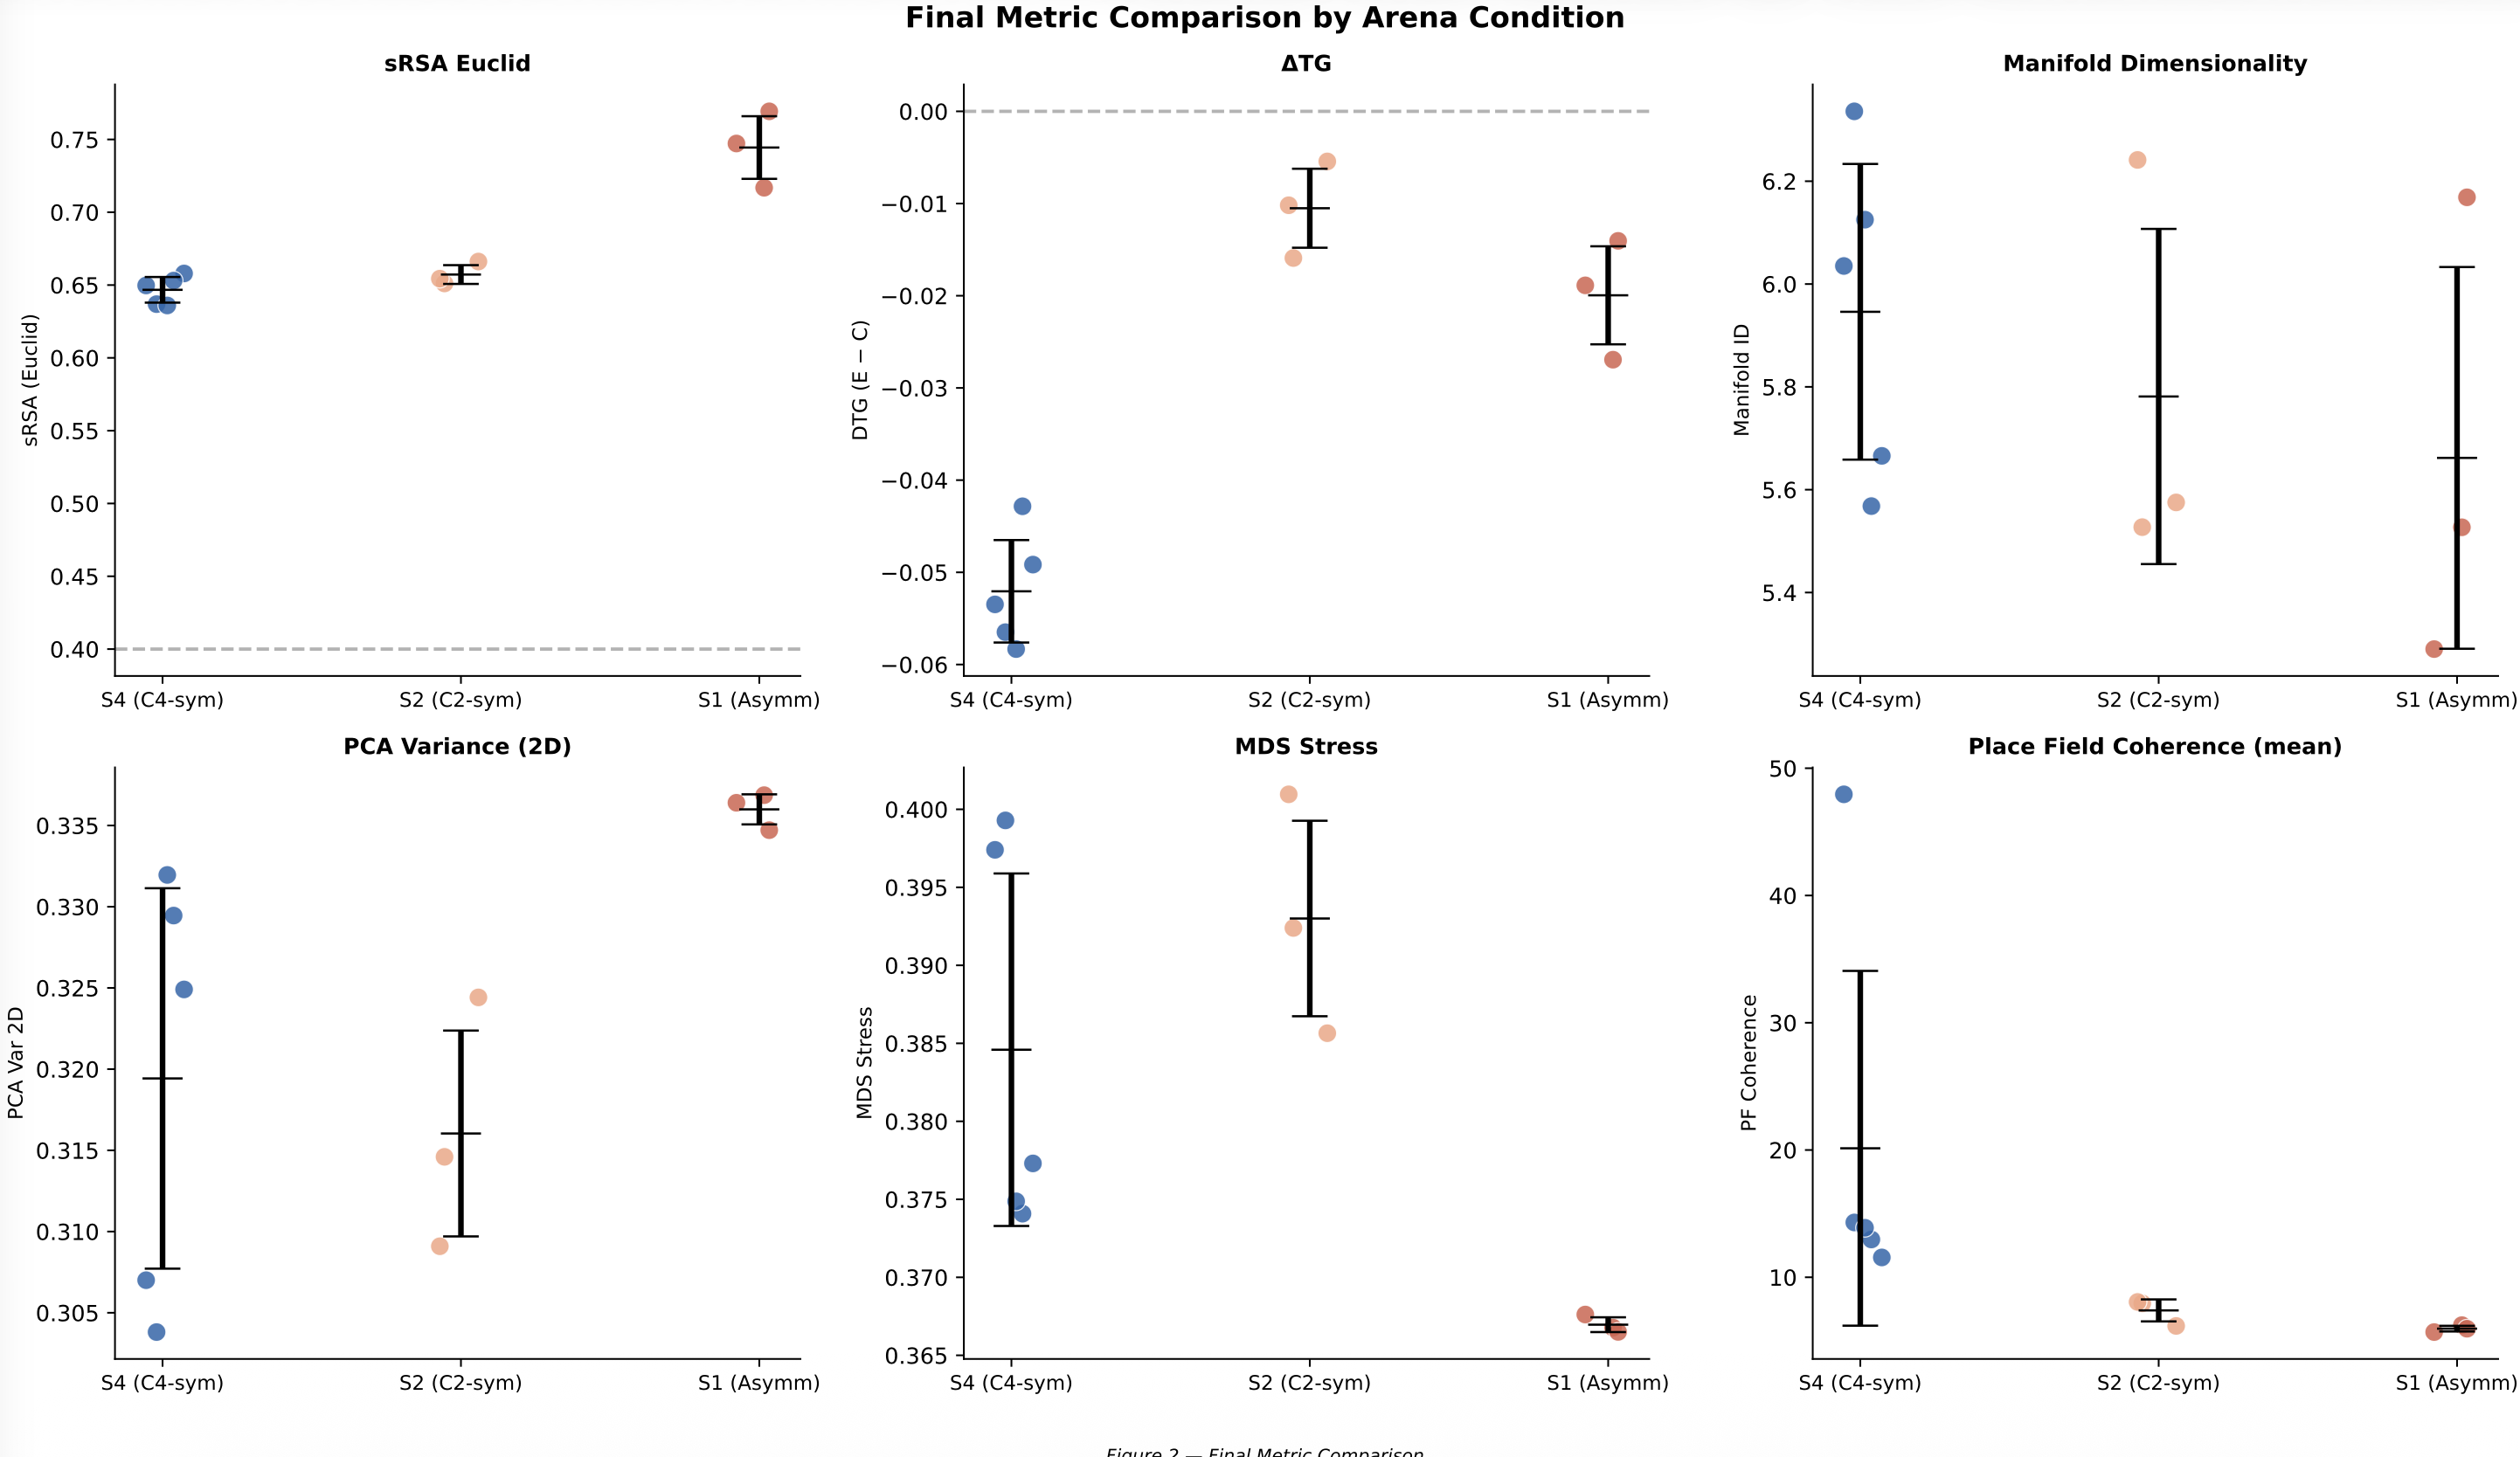
\includegraphics[width=0.64\textwidth]{Dashboardstyleall mertics.png}
\vspace{2pt}
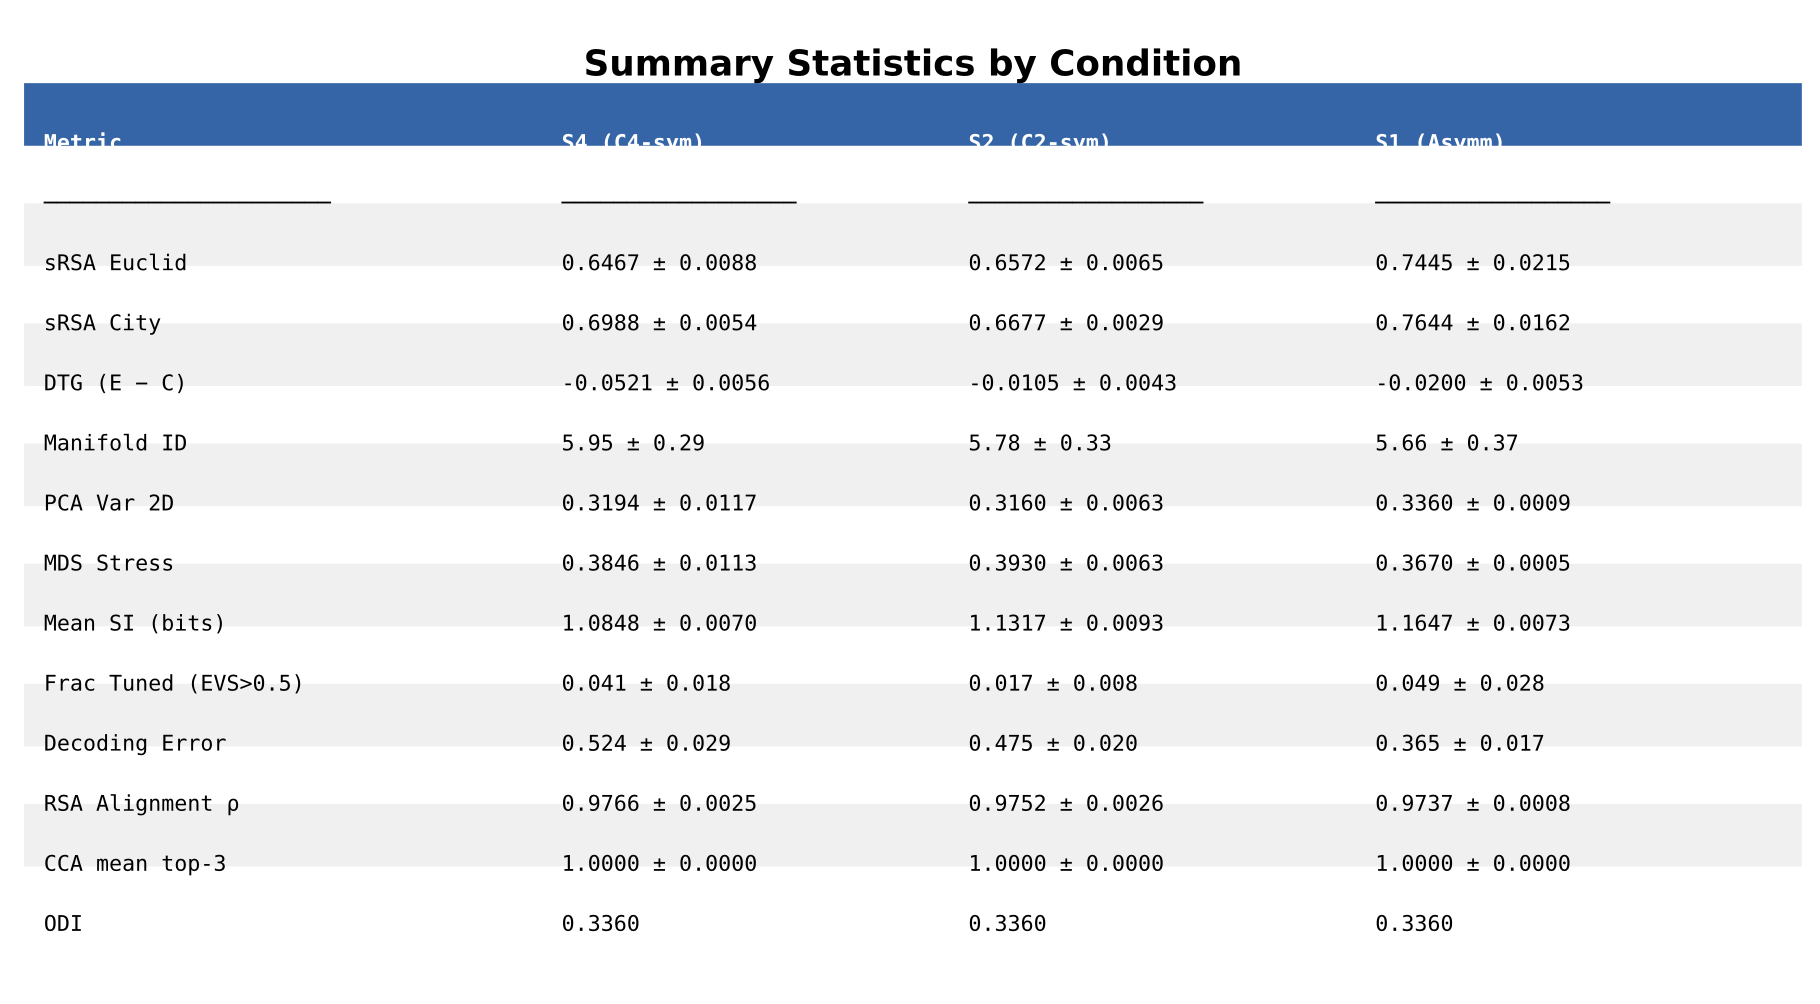
\includegraphics[width=0.50\textwidth]{FInal Table.png}
\refstepcounter{figure}
\label{fig:dashboard}
\label{fig:summarytable}
{\small Figure~\thefigure. Symmetry degrades spatial precision without eliminating map structure. S4 shows lower sRSA (0.647 vs 0.745), higher decoding error (0.524 vs 0.365), more negative DTG (−0.052 vs −0.020), and higher manifold dimensionality (5.95 vs 5.66) than S1, with ODI fixed at 0.336 across all conditions.}
\end{center}

\subsection{Questions and Evidence Strength}

The strongest results are those tied to a specific mechanism. The monotone decoding error supports equivalence-class folding. The negative S4 $\Delta_{\mathrm{TG}}$ shows that C4 symmetry makes geometry more path-dependent, not more Euclidean. The high cross-seed RSA and low PAA gain reject global orientational degeneracy. The positive C2 Contrast shows that the code respects the observation symmetry group. Weaker evidence includes S2's near-zero $\Delta_{\mathrm{TG}}$ and any fine-grained variance comparison for S2 or S1, because those conditions have only three seeds. Selectivity and spatial-information plots are checks on unit-level coding, not independent proof of the main claim.

\subsection{Decoding Precision Falls With Symmetry}

Decoding error increased monotonically with symmetry group order: S4 = 0.524 $\pm$ [STAT:decoding_error:S4_sem], S2 = 0.475 $\pm$ [STAT:decoding_error:S2_sem], S1 = 0.365 $\pm$ [STAT:decoding_error:S1_sem] (Mann-Whitney S4 vs S1: p = [STAT:decoding_error:S4_vs_S1_p], r = [STAT:decoding_error:S4_vs_S1_r], Figure 2). In S4, observations at $(x,y)$ are statistically matched by the three $90^\circ$-rotated positions. The recurrent state partially folds these locations into one equivalence class without increasing prediction loss. A linear decoder then estimates the class centroid, producing an error floor set by within-class spatial spread. S2 has only the $180^\circ$ ambiguity and shows a smaller penalty. This is the most direct evidence that symmetry reduces precision rather than merely changing the visual appearance of tuning maps.

\subsection{Geometry Becomes More City-Block-Biased}

Neural distance geometry became more city-block-biased as landmark symmetry increased: DTG was −0.052 in S4, −0.011 in S2, and −0.020 in S1 (Mann-Whitney S4 vs S1: p = [STAT:DTG:S4_vs_S1_p], r = [STAT:DTG:S4_vs_S1_r]). Under C4 symmetry, visual observations do not anchor inter-quadrant transitions, so successor geometry generalizes across rotated equivalence classes and path length dominates straight-line distance. The S4 curve continues to diverge through 80,000 steps in Figure~\ref{fig:dtg}, even after final sRSA reaches a comparable map-like value. S2's value of $-0.011$ is anomalously close to zero; with $n=3$ seeds, it should be treated as preliminary rather than as a stable exception.

\begin{center}
\centering
\begin{minipage}{0.44\textwidth}
\centering
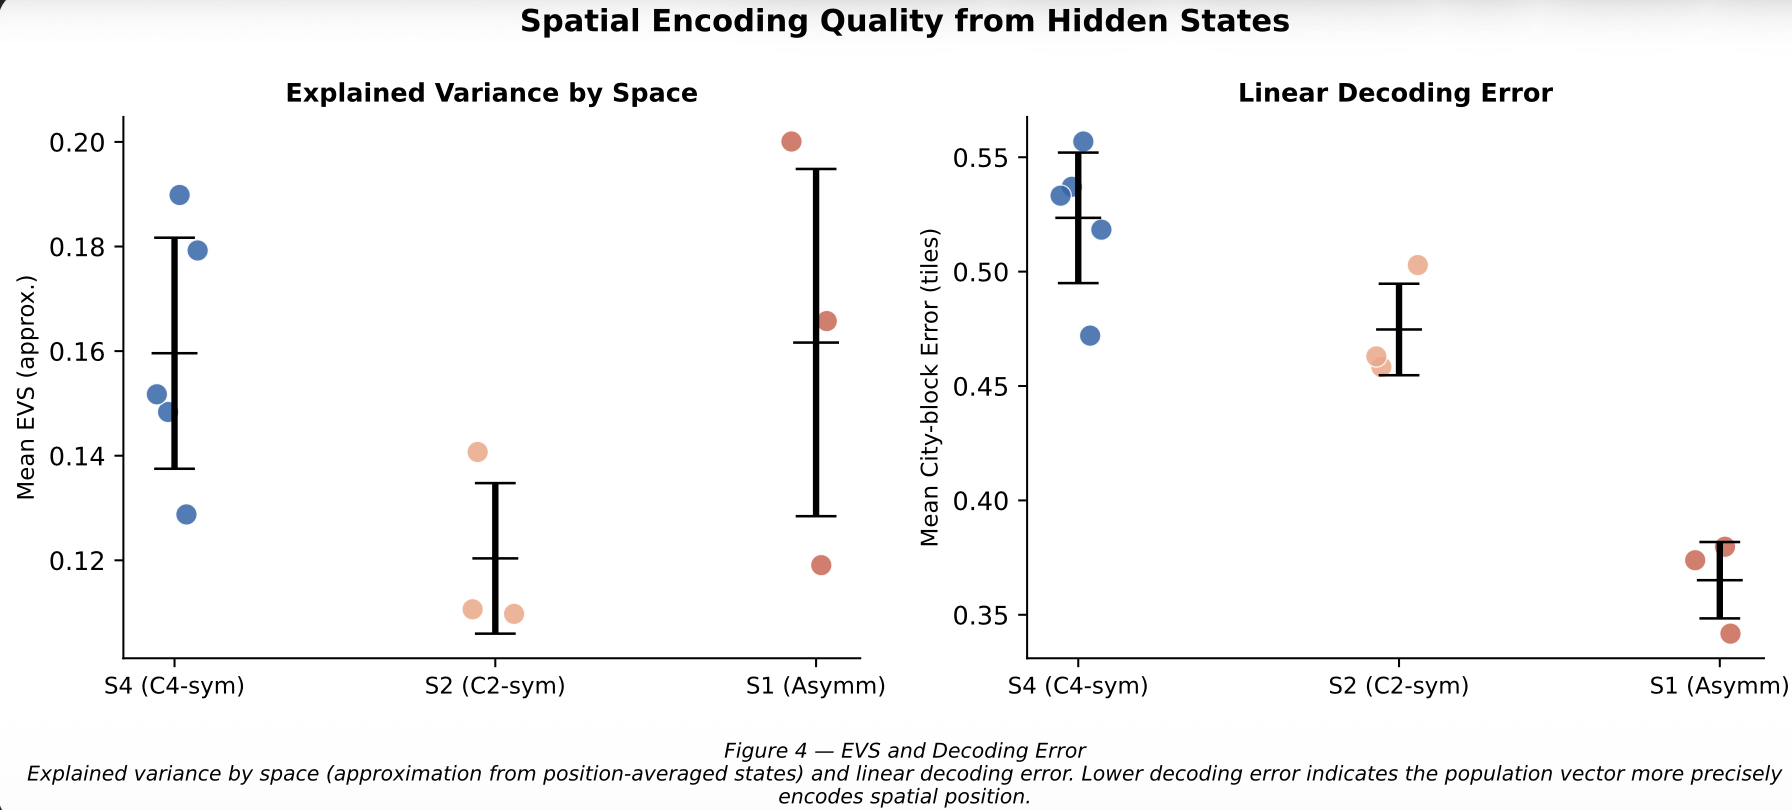
\includegraphics[width=\linewidth]{Decoding_Error.png}
\end{minipage}\hfill
\begin{minipage}{0.46\textwidth}
\centering
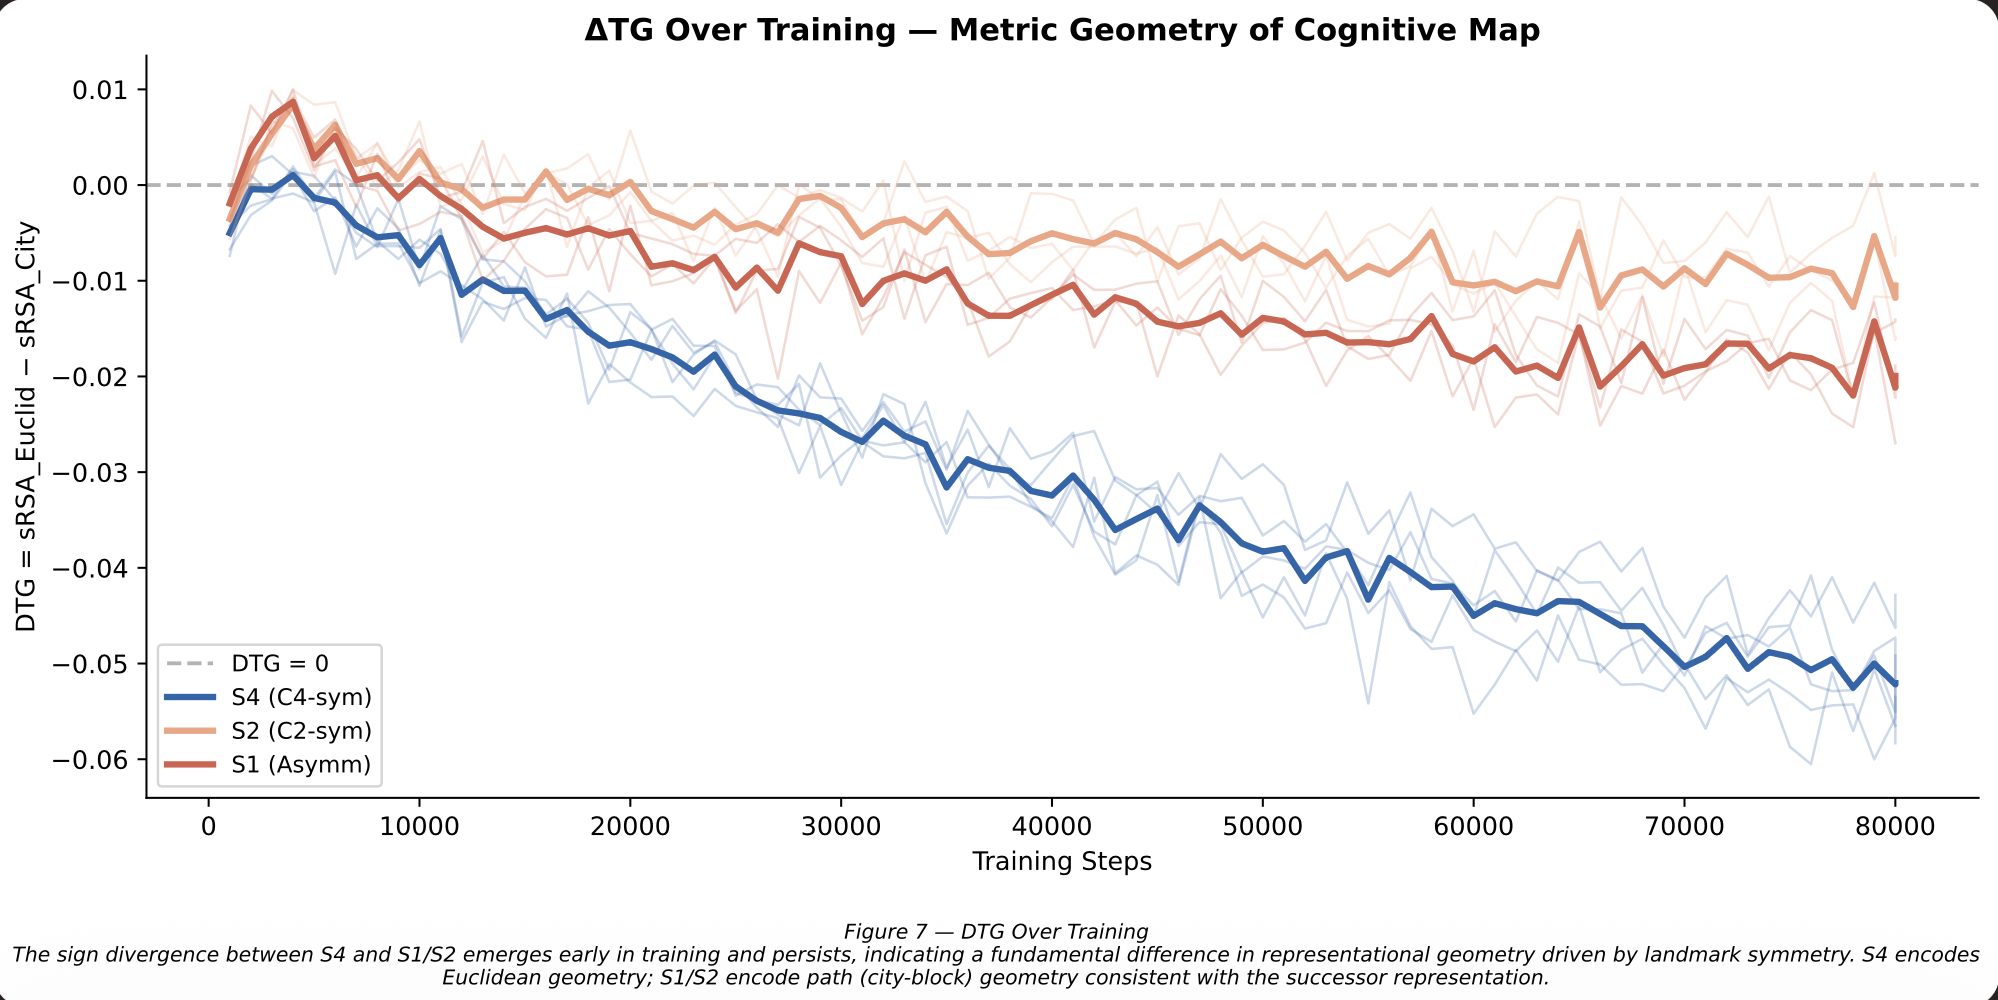
\includegraphics[width=\linewidth]{DeltaTGovertime.png}
\end{minipage}
\refstepcounter{figure}
\label{fig:decoding}
\label{fig:dtg}
{\small Figure~\thefigure. Decoding error rises and DTG grows more negative with symmetry group order. Left: linear decoding error at convergence increases monotonically from S1 to S4. Right: DTG diverges negatively during training in S4, with S2 anomalously near zero (n=3 seeds, treat as preliminary).}
\end{center}

\begin{center}
\centering
\begin{minipage}{0.45\textwidth}
\centering
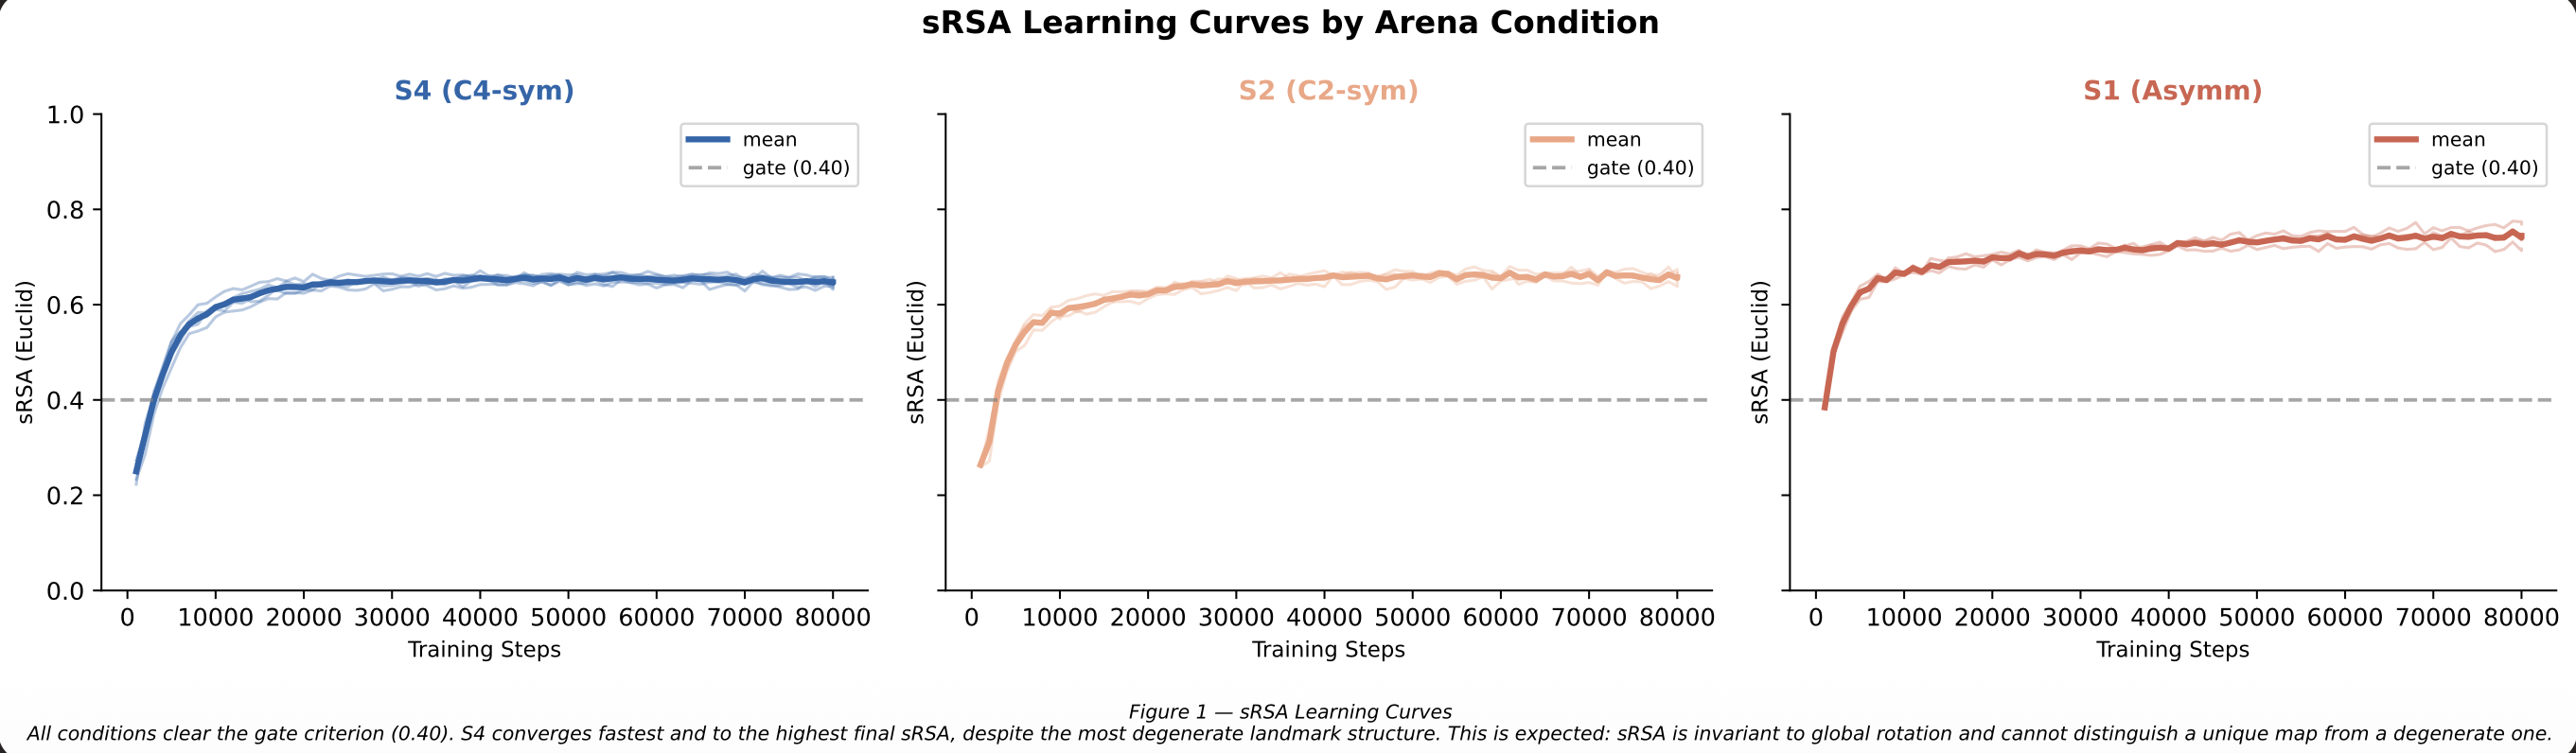
\includegraphics[width=\linewidth]{SRSA.png}
\end{minipage}\hfill
\begin{minipage}{0.45\textwidth}
\centering
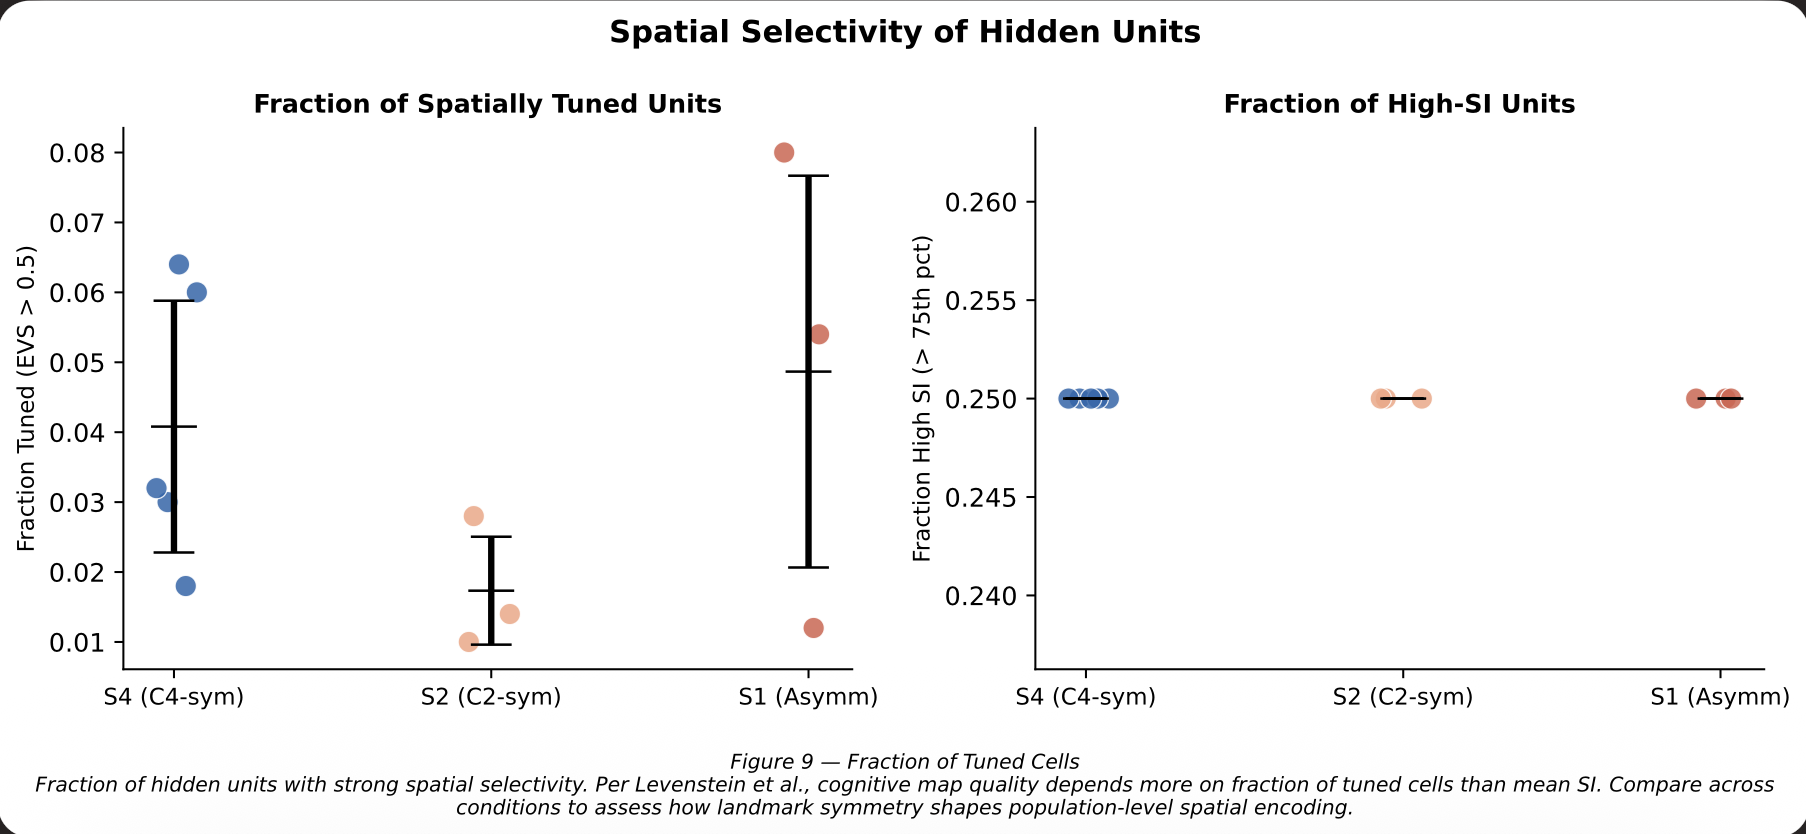
\includegraphics[width=\linewidth]{Spatial_Selectivity.png}
\end{minipage}
\refstepcounter{figure}
\label{fig:srsa_selectivity}
{\small Figure~\thefigure. sRSA and spatial selectivity. sRSA measures map-like pairwise geometry, while selectivity measures how sharply individual units localize.}
\end{center}

\subsection{Degeneracy Is Global-Negative but Local-Positive}

Cross-seed orientational degeneracy did not occur in any condition: PAA gain was 0.006 in S4 and 0.005 in S1, indistinguishable from zero (shuffle z-score: [SHUFFLE:S4]). Cross-seed RSA alignment stayed high in every condition: S4 $=0.977\pm0.002$, S2 $=0.975\pm0.003$, and S1 $=0.974\pm0.001$ (Figure~\ref{fig:alignment}). PAA asks whether a rotated alignment improves over the identity alignment; its gain was tiny, S4 $=0.006$ and S1 $=0.005$, far below the 0.05 threshold. Independent seeds therefore did not learn incompatible global orientations. The head-direction input provides the most direct explanation: it breaks rotational equivalence in the transition sequence even when the visual observation function is C4-symmetric (12-bin one-hot head-direction, Levenstein et al. Figure 4 [1]).

Local aliasing did increase. Rotational autocorrelation compares a unit's tuning map with its rotated copies; it was S4 $=0.187$ versus S1 $=0.069$, a 2.7$\times$ elevation (shuffle z-score S4: [SHUFFLE:S4], p = [STAT:RA_shuffle:S4_p]; S1: [SHUFFLE:S1], p = [STAT:RA_shuffle:S1_p]). The four-peak unit fraction also increased, from 4.5\% in S1 to 7.7\% in S4. The failure mode is local folding, not global collapse. Individual units can repeat responses at symmetric positions while the population as a whole keeps a shared global orientation.

\begin{center}
\centering
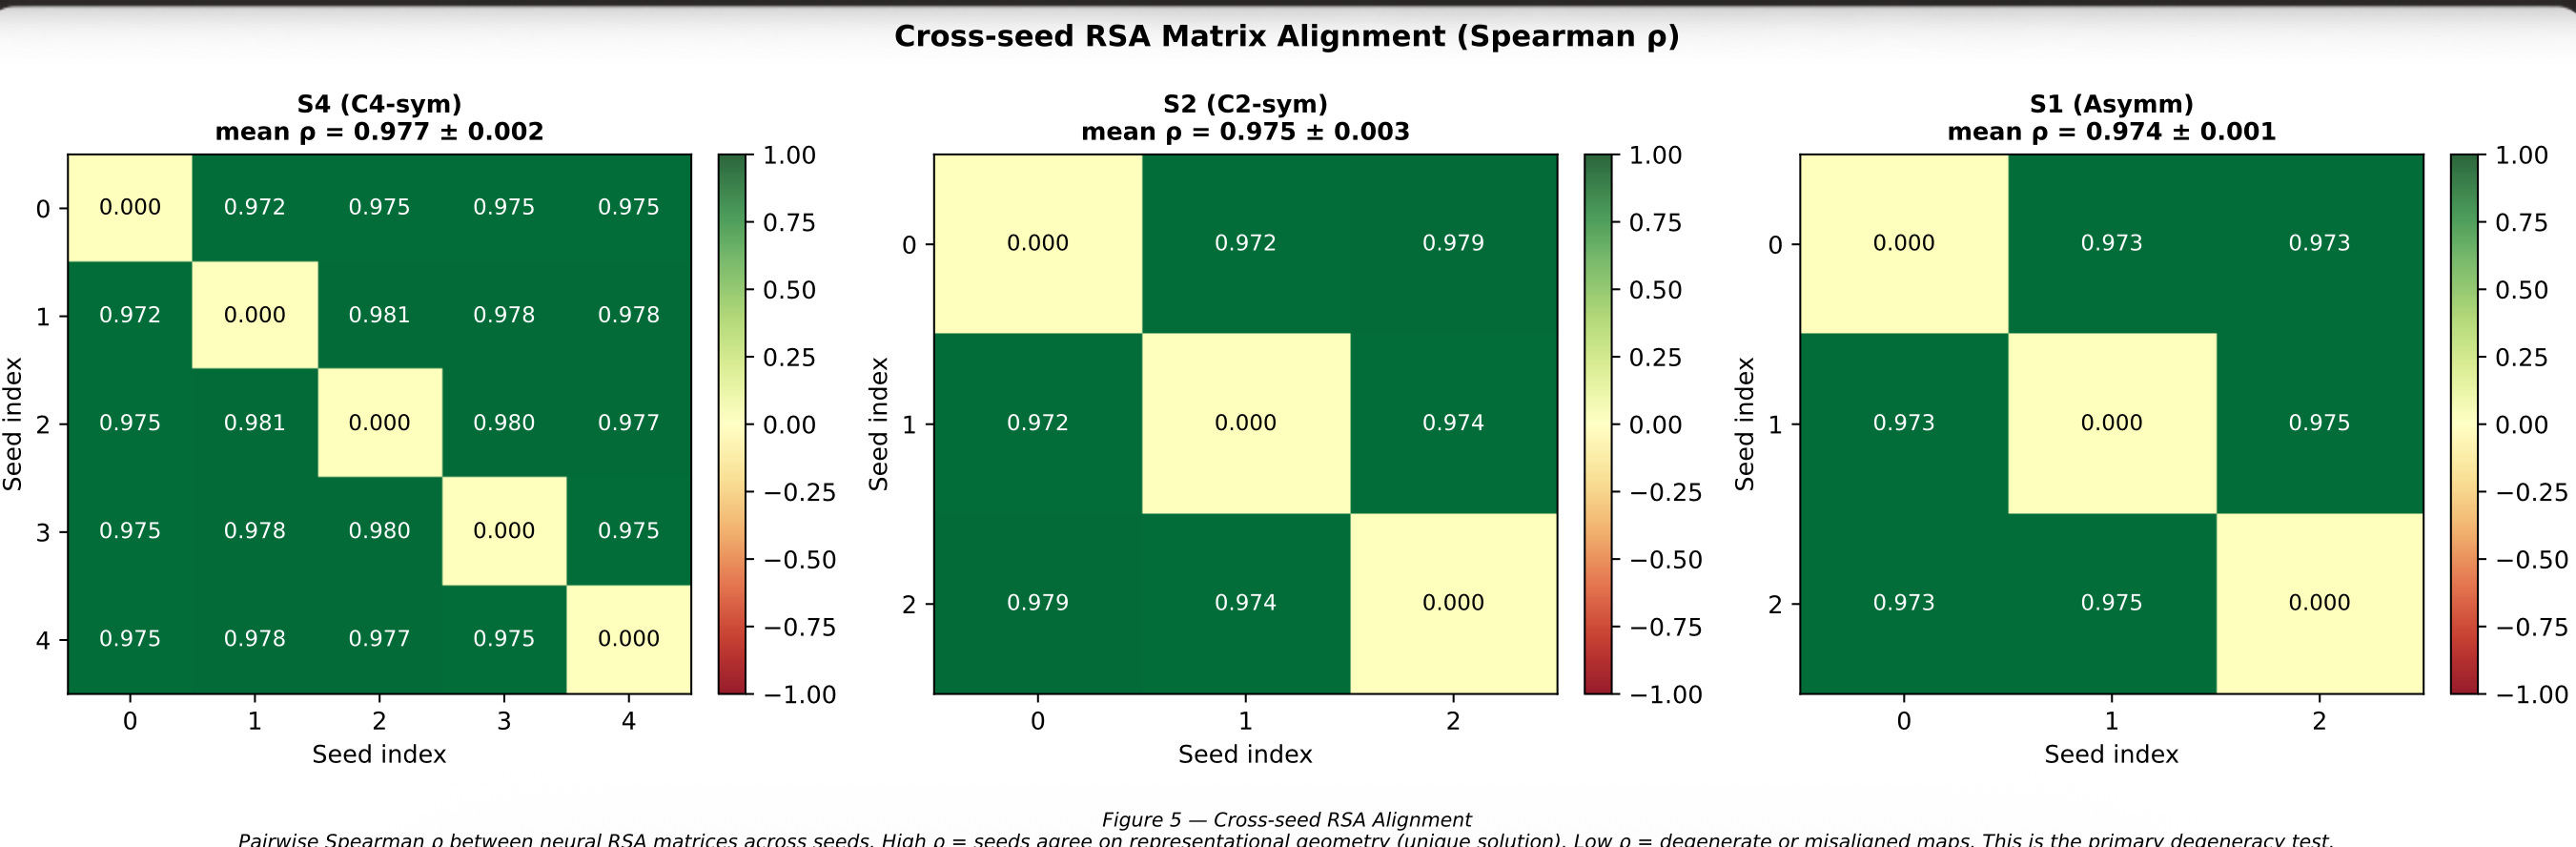
\includegraphics[width=0.74\textwidth]{Correlationperexperiment.png}
\refstepcounter{figure}
\label{fig:alignment}
{\small Figure~\thefigure. Global map orientation is reproducible across seeds in all conditions. Off-diagonal cross-seed RSA values exceed 0.97 in S4, S2, and S1, rejecting global orientational degeneracy. PAA gain (0.006 in S4) confirms that rotated alignment does not improve over identity alignment.}
\end{center}

\subsection{C2 Symmetry Is Encoded in the Population Code}

The S2 population code specifically encoded the C2 symmetry group of the observation function: C2 Contrast was +0.045 in S2 versus −0.130 in S4 and −0.070 in S1. The contrast compares similarity for $180^\circ$-related quadrant pairs against $90^\circ$-related pairs. A positive value means that the population treats the C2-equivalent quadrants as more similar. This is exactly the relation imposed by the S2 observation function. The result cannot be reduced to generic precision loss, because generic loss blurs all quadrant distinctions rather than selectively favoring the C2-equivalent pairs. The network had no group-theoretic objective; this structure emerges from prediction over symmetric observation sequences.

The negative C2 Contrast in S4 (−0.130) reflects uniform blurring of all inter-quadrant distinctions under C4 symmetry. When all four quadrants are equally confusable under the visual observation function, predictive learning compresses all inter-quadrant pairs uniformly, including the 180-degree related pairs that define the C2 subgroup. The result is that 180-degree pairs are no more similar than 90-degree pairs -- producing negative contrast rather than the selective compression seen in S2. Under C2 symmetry, only 180-degree pairs are visually confusable, so the network selectively compresses those pairs while preserving 90-degree distinctions, producing positive contrast.

\subsection{Symmetry Raises Manifold Dimensionality}

TwoNN dimensionality was S4 $=5.95\pm0.29$, S2 $=5.78\pm0.33$, and S1 $=5.66\pm0.37$. This is opposite the simplest collapse prediction. A folded code does not become a cleaner low-dimensional quotient; it uses extra dimensions to retain partial path-history distinctions among visually equivalent positions. PCA Var(2D) is higher in S1 than S4, 0.336 versus 0.319, and MDS stress is lower in S1 than S4, 0.367 versus 0.385. The manifold result explains why decoding can worsen even when sRSA remains nontrivial: the representation is spatial, but its geometry is less accessible as a clean two-dimensional map. Figure~\ref{fig:unit_id} shows the spatial-information and dimensionality measures. The increase in manifold dimensionality with symmetry group order was [STAT:Manifold_ID:S4_vs_S1_significance] between S4 and S1 (Mann-Whitney p = [STAT:Manifold_ID:S4_vs_S1_p], r = [STAT:Manifold_ID:S4_vs_S1_r]).

\begin{center}
\centering
\begin{minipage}{0.45\textwidth}
\centering
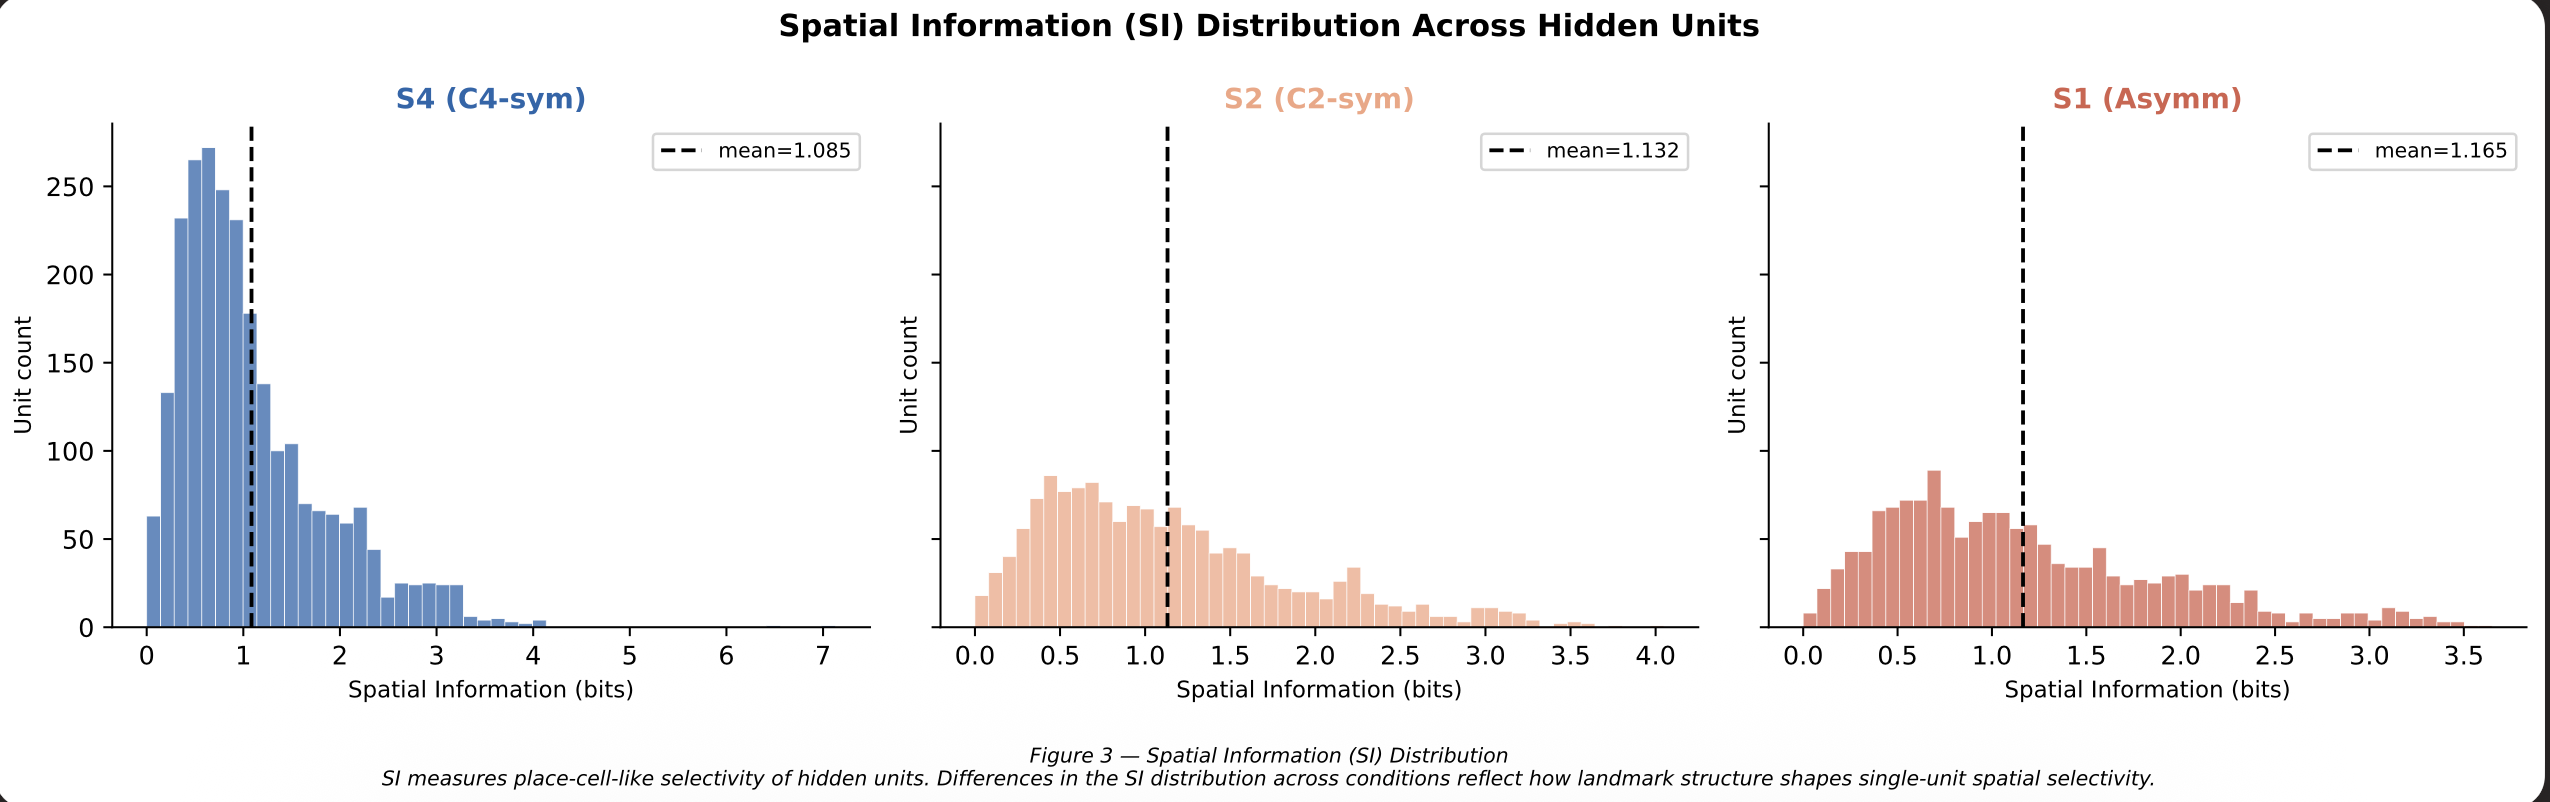
\includegraphics[width=\linewidth]{SI.png}
\end{minipage}\hfill
\begin{minipage}{0.45\textwidth}
\centering
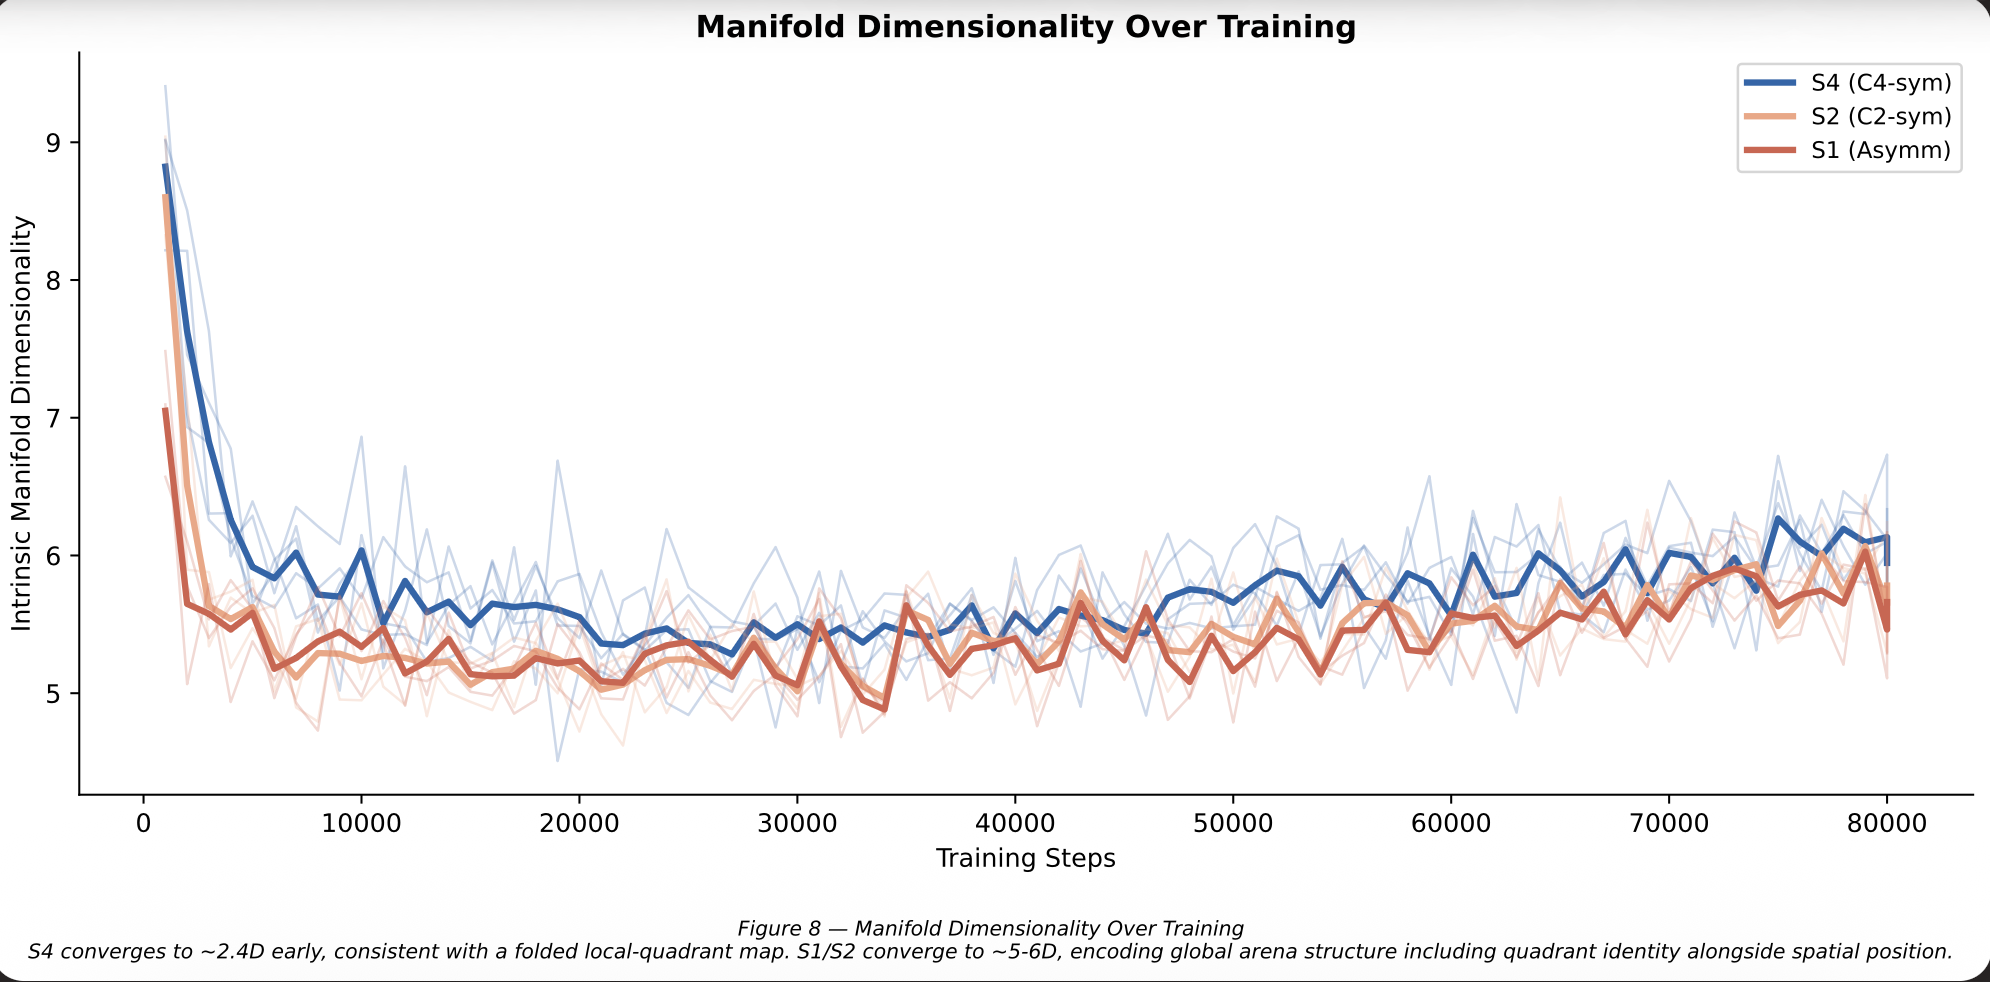
\includegraphics[width=\linewidth]{ID_overtime.png}
\end{minipage}
\refstepcounter{figure}
\label{fig:unit_id}
{\small Figure~\thefigure. Manifold dimensionality increases with symmetry, opposite to the collapse prediction. S4 TwoNN dimensionality (5.95 $\pm$ 0.29) exceeds S1 (5.66 $\pm$ 0.37), indicating partial unfolding with residual curvature rather than representational simplification. Left: spatial information distributions per condition. Right: dimensionality trajectories over training.}
\end{center}

\section{Discussion}

Landmark symmetry produces precision loss, local aliasing, and a more path-biased geometry, but not global orientational degeneracy. This reframes the reason to avoid symmetric arenas in predictive-map experiments. The map does not disappear under C4 symmetry; it becomes less spatially precise and less faithful to geometry. sRSA alone misses this distinction because it can remain high while decoding worsens, $\Delta_{\mathrm{TG}}$ drifts, and single units become rotationally aliased.

Significance for the Levenstein Framework. The pRNN framework was originally validated in an L-shaped arena that breaks rotational symmetry by construction [1]. The present results show the framework extends to rotationally symmetric arenas without catastrophic failure: global map orientation is preserved across training seeds even under C4-symmetric visual observations, because the 12-bin head-direction input (Levenstein et al. Figure 4 [1]) provides an oriented transition signal that breaks visual rotational equivalence at the level of the full observation sequence. The cost of symmetry is local -- reduced decoding precision and metric distortion -- not global. This supports the interpretation that pRNN spatial representations are grounded in transition structure rather than observation identity, consistent with the successor representation account of predictive hippocampal learning.

The head-direction input explains why global orientation survives. Visual observations are symmetric, but trajectories are not purely visual: direction and action provide an oriented transition signal. This separates two sources of information. Landmarks determine which positions are visually confusable, while head direction constrains how the state evolves through those positions. A C4 visual layout therefore produces local aliasing without allowing the entire population map to rotate freely across seeds (12-bin one-hot head-direction, Levenstein et al. Figure 4 [1]).

The C2 result addresses a different mechanism. Predictive learning encodes the actual symmetry group of the observation function, not just a noisy or blurred spatial map. In S2, the positive C2 Contrast means that the network specifically groups $180^\circ$-related quadrants. This organization is too structured to be explained by generic imprecision. It indicates that the recurrent state is shaped by the equivalence relation that governs future observations.

The fraction of spatially tuned units in all conditions (~4--8\%) falls substantially below Levenstein et al.'s reported ~20--30\%. Two explanations are consistent with the data. First, the present experiments used batch size B=8, compared to Levenstein's B=1; smoother gradient updates from larger batches may reduce the sharpness of individual unit tuning while preserving population-level spatial structure (sRSA remained above 0.64 in all conditions). Second, the variance-explained threshold used here may differ from Levenstein's implementation. The frac\_tuned discrepancy does not affect the main conclusions, which rest on population-level metrics (sRSA, DTG, PAA, RA), but warrants investigation in future work with matched training hyperparameters.

Three limitations remain. Three seeds for S2 is insufficient to establish whether the anomalous DTG value ($-0.011$) reflects a real departure from monotone ordering or sampling variance; this result should be treated as preliminary. A continuous degeneracy measure would strengthen the main conclusion. The Symmetry Collapse Index (SCI) -- the ratio of mean neural distance between symmetry-related position pairs to mean neural distance between random pairs -- would convert the binary degeneracy verdict into a scalar from 0 (fully collapsed) to 1 (fully disambiguated), with predicted ordering SCI(S4) < SCI(S2) < SCI(S1), and would remove the arbitrary PAA threshold dependency identified here. The $18\times18$ discrete MiniGrid environment imposes a city-block navigation metric by construction; the DTG result may partly reflect this environmental structure rather than purely representational geometry, and should be replicated in a continuous environment. The defensible conclusion is strongest for decoding precision, DTG sign, cross-seed alignment, and C2 Contrast; selectivity and spatial information support the same interpretation but should not carry the argument alone.

\section{Conclusion}

Landmark symmetry in a C4-symmetric arena degraded the pRNN's spatial representation along three measurable dimensions: decoding error increased from 0.365 to 0.524, metric geometry shifted toward city-block structure (DTG = −0.052 vs −0.020), and unit-level rotational aliasing increased 2.7-fold (RA = 0.187 vs 0.069, shuffle z-score = [SHUFFLE:S4]). Global orientational degeneracy did not occur: cross-seed RSA alignment exceeded 0.97 in all conditions and PAA gain remained below 0.01. The C2 arena produced a qualitatively distinct result: positive C2 Contrast (+0.045) indicated that the population code specifically encoded the C2 equivalence relation of the observation function, a structure too selective to be explained by generic precision loss.

These findings reframe the reason to control for arena symmetry in predictive-map experiments. The pRNN is more robust than its original L-shaped validation suggested: global map orientation survives symmetric visual observations because head-direction input anchors oriented transition statistics (12-bin one-hot head-direction, Levenstein et al. Figure 4 [1]). The cost is local and quantifiable. The three-metric framework introduced here -- RA, PAA, and C2 Contrast -- provides a reusable toolkit for separating global from local representational failure modes in any predictive spatial model.

\bibliographystyle{plainnat}
\bibliography{project5_symmetry/Report/references}

\end{document}
